\documentclass{beamer}
\usepackage{biblatex}
\addbibresource{deck.bib}

\usetheme{Samhitha}

\title{Deep dive into Machine learning by leveraging Networks}
\subtitle{WE Machine Learning Project}
\author{Aarushi Gulati, Samhitha Bharthulwar, Saumya Chaturvedi}
\institute{WE Program Cohort 4}
\date{\today}

\begin{document}

\begin{frame}
\titlepage
\end{frame}


\begin{frame}{Project Idea}
    \begin{center}
        {\large \textbf{A deep dive into knowledge graphs and GNNs.}}
    \end{center}

    \begin{itemize}
        \item We've done basic ML 
        \item Graphs/Networks are very powerful - recommeder systems, PageRank, AlphaFold, drug side effects, traffic prediction, weather forecasting
        \item Modelling relation data
        \item Generate powerful, useful visual representations
    \end{itemize}
\end{frame}

\begin{frame}{Getting familiar with some terms}
    \textbf{Heterogenous graph}: A graph with multiple types of nodes and/or relations.
    \begin{figure}
        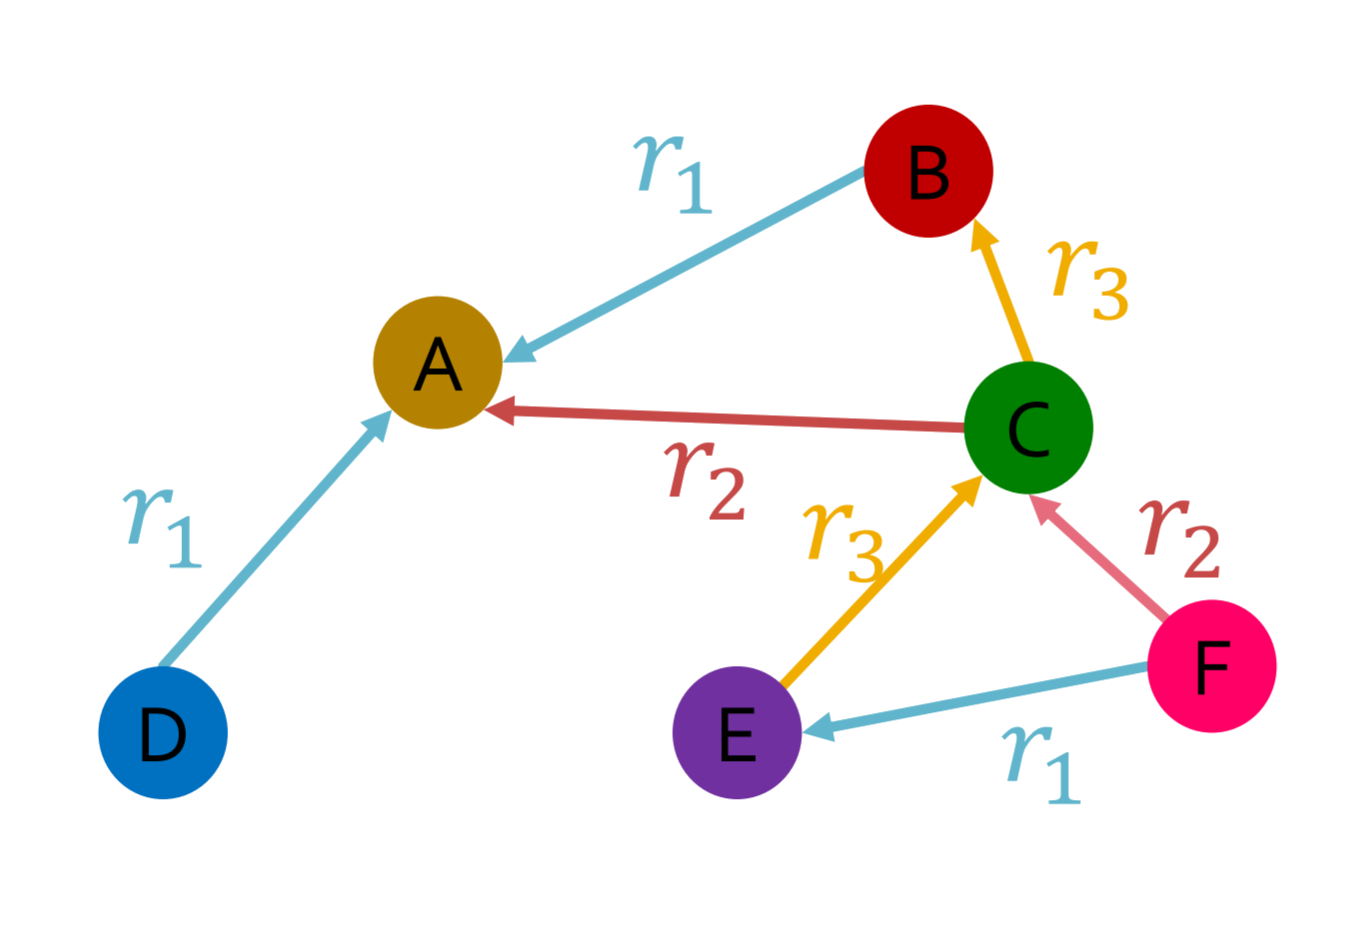
\includegraphics[width=0.5\textwidth]{attachments/diagram_heterogenous_graph.png}
        \caption{An example of a heterogenous graph \cite{course}}
        \label{fig:hg}
    \end{figure} 
\end{frame}

\begin{frame}{Getting familiar with some terms}
    \textbf{Knowledge graph}: A heterogenous graph where nodes represent entities and are labelled with types, and edges capture the relation between entities.
    \begin{figure}
            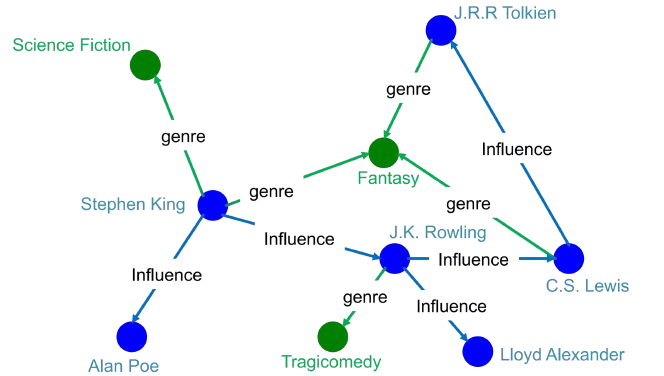
\includegraphics[width=0.7\textwidth]{attachments/diagram_kg.png}
            \caption{An example of a knowledge graph \cite{course}}
            \label{fig:kg}
    \end{figure}
\end{frame}


\begin{frame}{Current Progress}
    \begin{itemize}
        \item Studying networks \cite{course}
        \item Key steps in building a knowledge graph - Named Entity Recognistion (NER) + Relation Classification (RC)
        \item Experimenting - REBEL, Mistral 7B, Llama
    \end{itemize}
\end{frame}

\begin{frame}{Learning Objectives}
    \begin{itemize}
        \item Represent data corpus through knowledge graphs \cite{paper}
        \item Explore Graph Visualisation techniques
        \item Work with Knowledge Graph Transformers
        \item Learn about networks and their properties
        \item Apply different graph neural networks
    \end{itemize}
\end{frame}

\begin{frame}{Strategy}
    \begin{itemize}
        \item Input: complex knowledge base
        \item Generate a knowledge graph: NER + RC 
        \item Visualisation
        \item Perform Link Prediction, Entity Classification
    \end{itemize}
\end{frame}

\begin{frame}{Next Steps}
    \begin{itemize}
        \item Continue exploring different ways to create KGs.
        \item Try different Graph Visualization methods. 
        \item Implement KG embeddings (using BERT KG and other Transformers).
        \item Learning about the working of GNNs.
    \end{itemize}
\end{frame}

\begin{frame}{Timeline}
    \begin{itemize}
        \item Bare minimum: KG creation + visualization + 1 GNN application
        \item Satisfactory: if we complete KG creation, visualization and application of 2-3 GNNs 
        \item Excelling: various applications with code and proper documentation for all 3 stages, while accomplishing 2-3 tasks with the dataset
    \end{itemize}
\end{frame}

\begin{frame}{References}
    \printbibliography
\end{frame}

\end{document}

% Suggestions:
% [-] Timeline
% [-] Diagrams
% [ ] Talk about the paper